\chapter{MVDR ABF polynomial zeros }
\label{ch:mvdr-polyn-zeros}
The $z$ transform of the conjugated weights of the ABF produce the ABF
array polynomial. Evaluating the ABF polynomial on the unit circle
yields the beampattern. The ABF polynomial zeros on the unit circle
are associated with the ABF beampattern nulls. The ABFs use the
knowledge of the operating environment to adjust the beampattern to
achieve optimal output. As the ABFs adjust the beampattern, the
associated ABF polynomial zeros also change location on the complex
plane. This chapter focuses on the ensemble MVDR ABF polynomial and
its zeros. The first section presents the ensemble MVDR ABF polynomial
and the properties of its zeros. The second section develops a model
for the location of the ensemble MVDR polynomial zeros as a function
of interferer power. The final section discusses the behavior of the
SMI MVDR ABF polynomial zeros.

\section{Ensemble MVDR ABF polynomial}
\label{sec:mvdr-polynomial}
The ensemble MVDR ABF polynomial is
$\mvdrpoly{z} = \ztrans(\wmvdr\herm)$ where $\ztrans(\cdot)$ denotes
the $z$ transform operation and $\wmvdr$ is the ensemble MVDR ABF
weight vector. Factoring the polynomial in terms of the zeros,
\[
\mvdrpoly{z}  =  \Gamma \prod\limits_{n=1}^{N-1}(1 - \ensz_n z\inv),
\]
where $\Gamma$ is a scaling term to ensure unity gain in the look
direction ($\ulook$), i.e., $\mvdrpoly{\expo{j\pi\ulook}} = 1$ and
$\ensz_n$ is the $n^{th}$ zero. The ensemble MVDR ABF polynomial zeros
will be referred to as ensemble zeros in the
sequel. \figurename{}~\ref{fig:mvdr-plots} shows the ensemble zeros
and log magnitude of the beampattern for an example case of the
ensemble MVDR ABF using $N = 11$ sensor ULA. A single interferer is
present at $\uinter = 3/N$ and the interferer-to-noise power ratio
(INR) is 10 dB. The dashed radial line in
\figurename{}~\ref{fig:mvdr-pzplot} indicates the phase angle
$\pi\uinter$ corresponding to the interferer direction
$\uinter$. Denote the unit circle point corresponding to the
interferer direction as $\interz = \expo{j\pi\uinter}$. In the complex
plane, all $10$ ensemble zeros fall on the unit circle. These unit
circle zeros produce the beampattern nulls seen in the log magnitude
beampattern plot \figurename{}~\ref{fig:cbf-mvdr-bpplot}. The vertical
dotted line in the beampattern plot indicates the interferer direction
($\uinter$).

\begin{figure}[!hp]
  \centering
  \subfloat[]{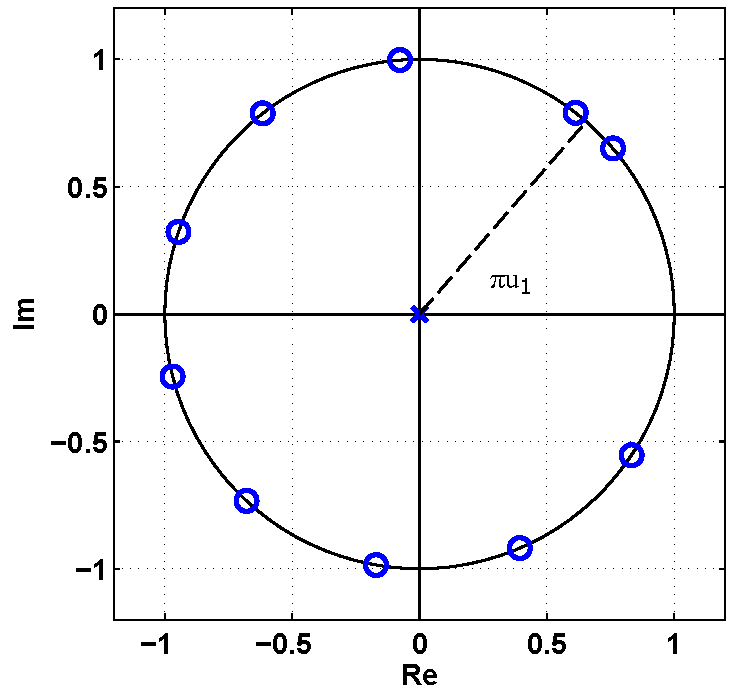
\includegraphics[width=3.5in]{mvdr_cbf_pzplot_N11_INR0}
    \label{fig:mvdr-pzplot}} \hfill
  \subfloat[]{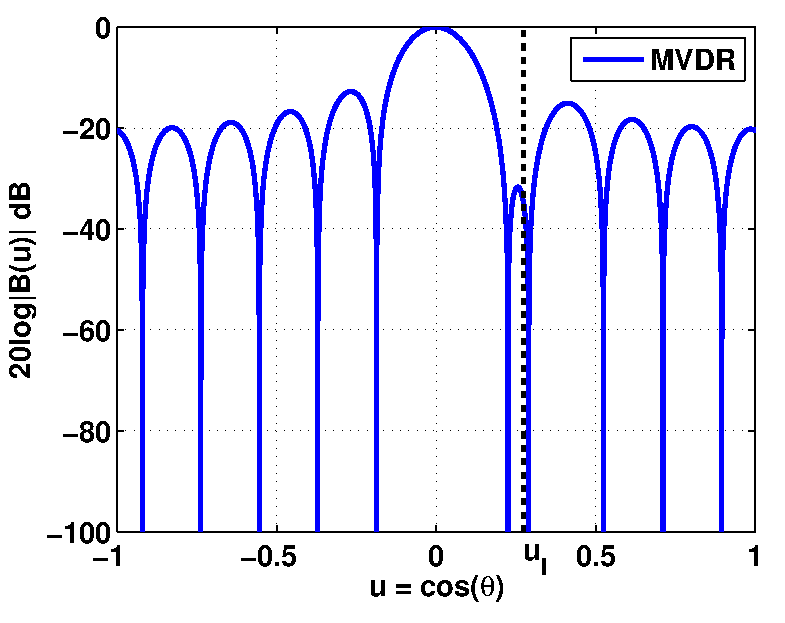
\includegraphics[width=3.5in]{mvdr_cbf_N11_bp_plot}
  \label{fig:cbf-mvdr-bpplot}}
\caption[Ensemble MVDR ABF \protect\subref{fig:mvdr-pzplot} polynomial
  zero locations and \protect\subref{fig:cbf-mvdr-bpplot} log
  magnitude of beampattern for an example case using $N = 11$ sensor
  ULA.]{Ensemble MVDR ABF \protect\subref{fig:mvdr-pzplot} polynomial
  zero locations and \protect\subref{fig:cbf-mvdr-bpplot} log
  magnitude of beampattern for an example case using $N = 11$ sensor
  ULA. A single interferer is present at $\uinter = 3/N$ indicated by
  vertical dashed line in \protect\subref{fig:cbf-mvdr-bpplot}. In
  \protect\subref{fig:mvdr-pzplot} the dashed radial line at indicates
  the phase angle $\pi\uinter$. The ensemble zeros are constrained on
  the unit circle and produce nulls in the beampattern.}
  \label{fig:mvdr-plots}
\end{figure}

Expanding to a multiple planewave interferer case, numerical
experiments found that the ensemble zeros are still constrained to the
unit circle. 50000 independent ensemble MVDR weight vectors were
generated for an $N = 11$ sensor ULA. In each scenario there were a
random number of interferers with counts ranging from
$1~\text{to}~10$, at random locations between $-1\leq u \leq 1$ and
INR level randomly set between 10 to 40 dB. The ensemble zeros in all
50000 scenarios were on the unit circle. Repeating this experiment
with a $N = 41$ sensor ULA found the same result. In fact the MVDR
ensemble zeros are always constrained on the unit circle for planewave
beamforming using ULAs. Steinhardt and Guerci found similar behavior
of the ensemble zeros, but the result does not appear to be widely
known \cite{steinhardt2004stap}. Steinhardt and Guerci present a proof
for the unit circle constraint on MVDR ensemble zeros which is
restated in Appendix~\ref{sec:apdx-mvdr-zeros}.

% Remainder of the chapter considers the single interferer case?

\section{Ensemble zero location on the unit circle}
\label{sec:mvdr-interf-suppr}
The unit circle constrained ensemble zeros create $N-1$ nulls in the
beampattern. But the ensemble MVDR ABF does not necessarily place the
nulls in the interferer directions. Numerical experiments show that
the ensemble MVDR ABF places a null in the vicinity of the interferer
direction to produce a deep notch at the interferer
direction. \figurename{}~\ref{fig:mvdr-notch-zoom} shows a zoomed
section of the ensemble MVDR ABF beampatterns in the neighborhood of
the interferer direction ($\uinter$). The vertical solid line
indicates interferer direction. The three beampatterns correspond to
the ensemble MVDR ABFs implemented for INR levels of $5$ dB (solid),
$10$ dB (dashed) and $15$ dB (dash-dot). The ensemble MVDR ABF adapts
the notch depth (ND) at the interferer direction according to the INR
level as discussed in \sect{}\ref{sec:notch-depth}. As the INR
increases, the beampattern null shifts towards the interferer
direction yielding a deeper notch. As INR decreases, the beampattern
null shifts away from the interferer direction yielding a shallower
notch. The change in beampattern null direction is replicated as
change in the location of the corresponding ensemble zero on the unit
circle.

\begin{figure}[hp]
  \centering
  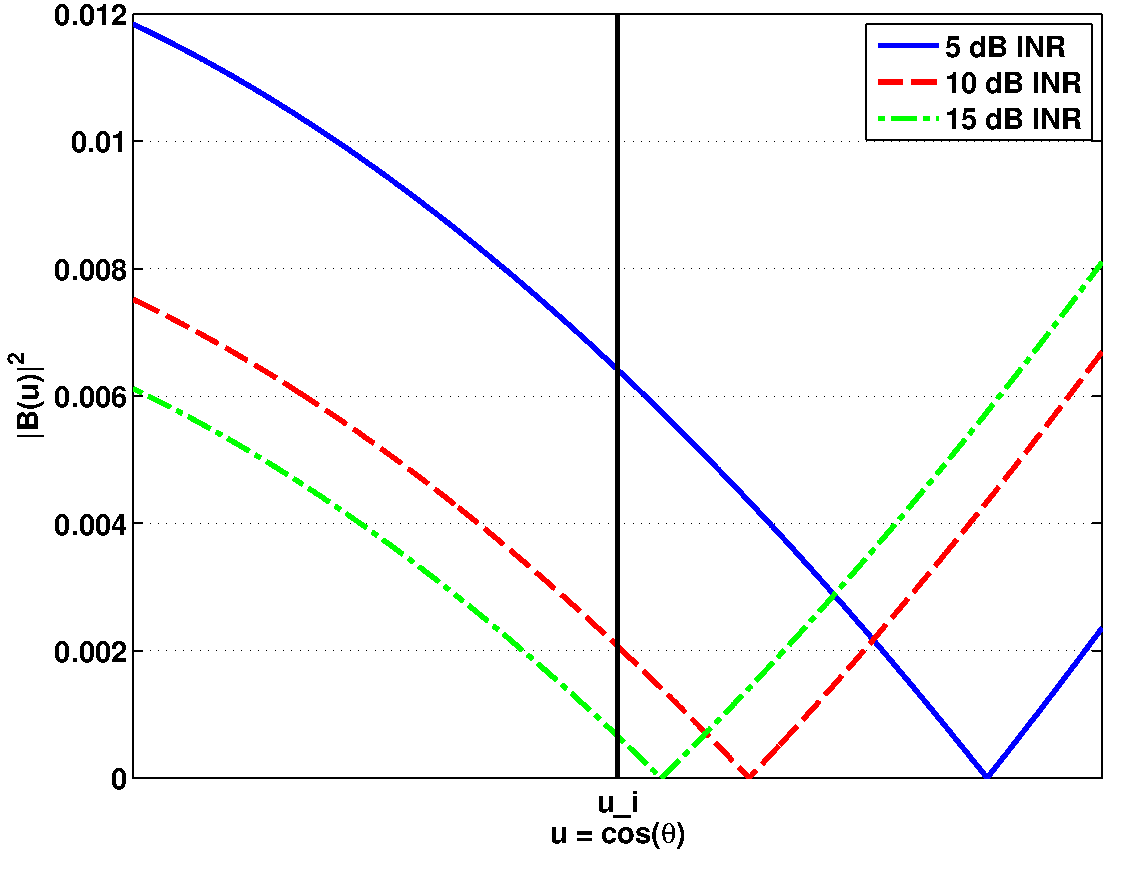
\includegraphics[width=1\textwidth]{single_interf_mvdr_bp_zoom.pdf}
  \caption[Zoomed in section of the ensemble MVDR ABF
    beampatterns.]{Zoomed in section of the ensemble MVDR ABF
    beampatterns. The ABF is implemented using $N = 11$ sensor ULA and
    a single interferer is present at $\uinter$. The solid vertical
    line denotes the interferer direction. The three beampatterns
    correspond to ensemble MVDR ABF implemented for the cases of INR =
    $5$ dB, $10$ dB and $15$ dB. The ensemble MVDR ABF adjusts the
    notch depth at the interferer direction by shifting the
    beampattern null closer to the interferer direction as the
    interferer power increases.}
  \label{fig:mvdr-notch-zoom}
\end{figure}

The ensemble zeros shift along the unit circle as the ensemble MVDR
ABF adjusts the beampattern to the interferer and the noise. Since the
ensemble zeros are constrained on the unit circle it is sufficient to
observe the phase angle of the ensemble zeros to examine their
location on the complex
plane. \figurename{}~\ref{fig:mvdr-zeros-phase} shows the phase angle
of the ensemble zeros as the INR changes from $-40$ dB to $40$ dB for
an example case of the ensemble MVDR ABF using an $N = 11$ sensor ULA
and steered towards broadside ($\ulook = 0$). A single interferer is
present at $\uinter = 3/N$. The solid curves denote the phase angle of
each of the $10$ ensemble zeros over the range of INR values. The
dashed horizontal line denotes the phase angle of the interferer point
$\interz = \expo{j\omega_I}$. The phase angle corresponding to the
look direction is $\omega_0 = 0$. The phase angles are expressed as
fraction of $\pi$ for convenience. For the following discussion,
denote the ensemble zero producing the black curve as $\ensz_1$ and
the ensemble zero producing to the magenta curve as $\ensz_2$. The
ensemble zeros $\ensz_1$ and $\ensz_2$ are the two zeros closest to
the interferer point.

As discussed in \sect{}\ref{sec:abf} the ensemble MVDR ABF simplifies
to the CBF for the case of zero interferer power. In
\figurename{}~\ref{fig:mvdr-zeros-phase}, for INR levels $< -20$ dB,
the solid curves are uniformly spaced in phase angle except at the
look direction phase angle. This uniform phase angle spacing indicates
that the ensemble zeros are approximately in the CBF polynomial zero
locations. As the INR increases the black curve and the magenta curve
shift towards the horizontal dashed line. This implies that the two
zeros $\ensz_1$ and $\ensz_2$ shift closer to the interferer point
($\interz$). Approximately beyond INR $> 10$ dB INR only the black
curve continues to move closer to the horizontal dashed line while the
magenta curve stop shifting. This implies that only the closest zero
($\ensz_1$) continues to move towards the interferer point for higher
INR values. Asymptotically as INR grows large, the ensemble zero
$\ensz_1$ approaches the interferer point $\interz$ and the ensemble
MVDR beamformer asymptotically places a null in the interferer
direction \cite{vtree2002oap}. Over the range of INR values examined
in \figurename{}~\ref{fig:mvdr-zeros-phase}, only two ensemble MVDR
polynomial zeros closest to the interferer change location with change
in INR level and the rest are approximately in the CBF polynomial zero
locations. In fact, at higher INR levels, only the closest ensemble
zero $\ensz_1$ is sensitive to the INR level. This suggests that for
strong interferers, the notch depth adaptation is dominated by the
single null corresponding to the ensemble zero
$\ensz_1$. Additionally, the continuous solid curves indicate that
each ensemble zero for a particular INR level has an associated CBF
polynomial zero location. The following section develops a model that
characterizes the phase angle of $\ensz_1$ as a function of the INR.

% the change in the closest zero $\ensz_1$ in terms of the perturbation
% of $\ensz_1$ from the interferer direction on the unit circle.

\begin{figure}[!hp]
  \centering
  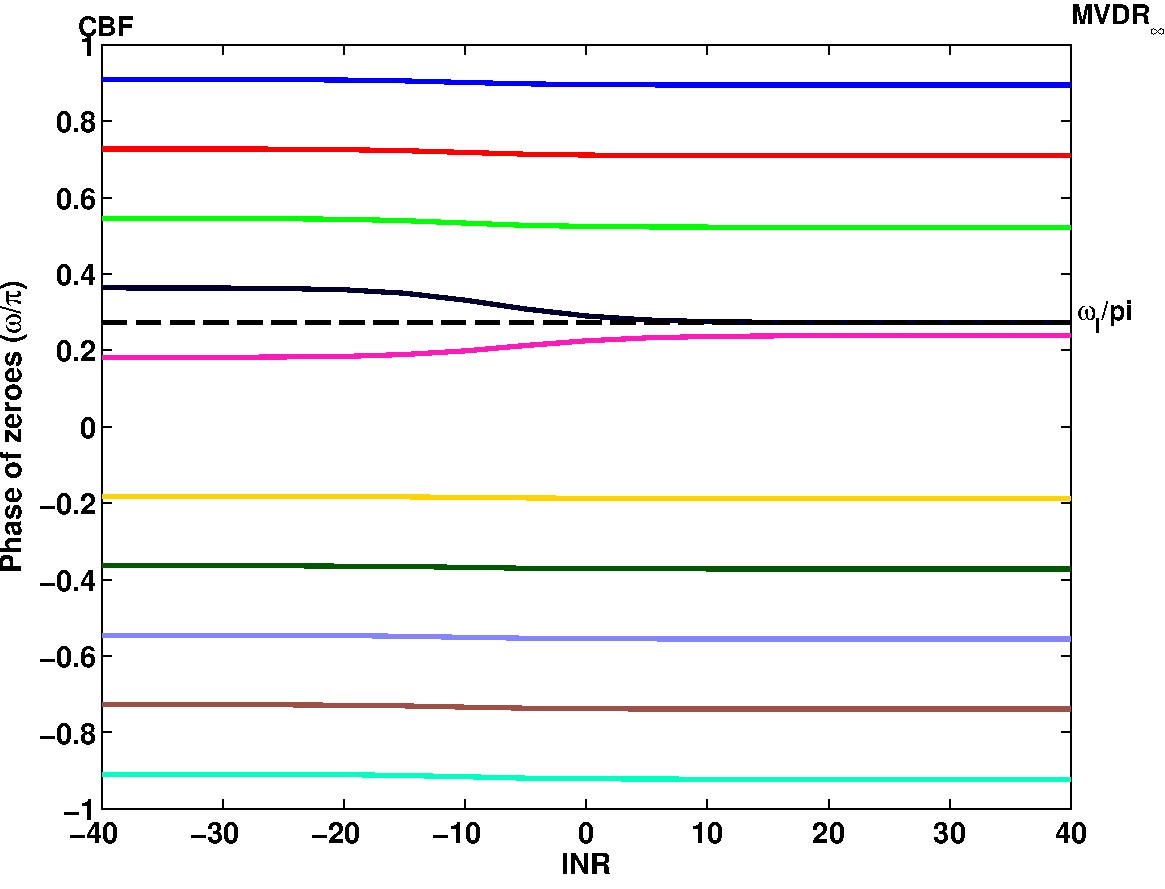
\includegraphics[width=6in]{mvdr_zeros_phase}
  \caption[Phase angle of the ensemble MVDR ABF polynomial
  zeros.]{Phase angle of the ensemble MVDR ABF polynomial zeros for a
    range of INR values. The ABF is implemented using an $N = 11$
    sensor ULA and a single interferer is present at $\uinter = 3/N$.
    The phase angle of the interferer direction is denoted by the
    horizontal dashed line. Only the ensemble zeros corresponding to
    the black and the magenta curve are sensitive to INR.}
  \label{fig:mvdr-zeros-phase}
\end{figure}

% =======================================================================
\section{Ensemble zero phase angle perturbation}
\label{sec:perturbation-model}
This section develops an approximate model for the location of the
ensemble zeros ($\ensz_n$) based on the observations in
\figurename{}~\ref{fig:mvdr-zeros-phase}. The model makes following
assumptions:
\begin{itemize}
\item A single strong interferer is present in the direction
  $\uinter$. The model focuses in the region where INR $\geq 10$ dB in \figurename{}~\ref{fig:mvdr-zeros-phase}.
\item Only the location of the ensemble zero closest to the interferer
  direction is sensitive to the INR level. The closest zero is denoted
  by $\ensz_1$. This model ignores the dependence of the second
  closest zero $\ensz_2$ on the INR, demonstrated by magenta curve in
  \figurename{}~\ref{fig:mvdr-zeros-phase}.
\item The remaining $N - 2$ ensemble zeros are approximated to be in
  the CBF polynomial zero positions. For a given ULA size, the CBF
  polynomial zero locations are known and independent of the INR level.\cite{vtree2002oap}.
\end{itemize}

\begin{figure}[!hp]
  \centering
  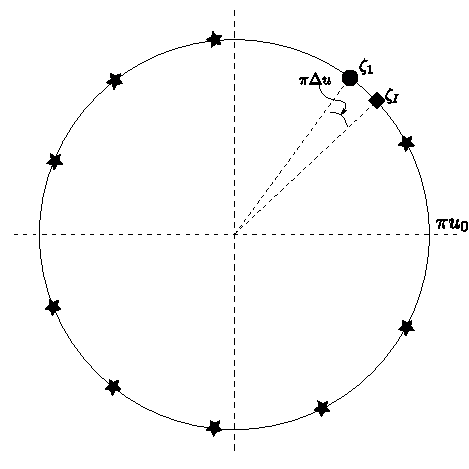
\includegraphics[width=6in]{unit_arc_zeros_pertb.pdf}
  \caption[Approximate model for ensemble zero locations.]{Approximate model for
    ensemble zero locations. The diamond marker denotes the interferer
    point ($\interz$) on the unit circle. The circle marker denotes
    the ensemble zero closest to the interferer and its location is
    expressed as phase angle perturbation of $\deltau$ from the
    interferer point. The phase angle perturbation $\deltau$ depends
    on the INR level. The star markers denote the CBF polynomial zeros
    which approximate the location of the remaining $N - 2$ ensemble
    zeros. The CBF polynomial zero locations are independent of the
    INR level.}
  \label{fig:perturb-model}
\end{figure}

\figurename{}~\ref{fig:perturb-model} shows the ensemble zero
configuration based on the assumptions stated above for the case of an
ensemble MVDR ABF implemented using a $N = 11$ sensor ULA. The diamond
marker denotes the interferer point ($\interz$) and the circle marker
denotes the ensemble zero $\ensz_1$. The phase angle of $\ensz_1$ is
defined as some perturbation from the interferer point phase angle,
i.e., $\ensz_1 = \expo{j\pi u_1} =\expo{j\pi(\uinter + \deltau)}$. The
phase angle perturbation $\deltau$ depends on the INR level. The star
markers denote the remaining $10$ ensemble zeros which are
approximated to be in the CBF zero locations. For a given number of sensors, the CBF polynomial zero locations are known and independent of the INR level. Based on the ensemble zero configuration in
\figurename{}~\ref{fig:perturb-model}, the ensemble MVDR ABF
polynomial is
\begin{align*} 
  \mvdrpoly{z} &\approx \left(\prod\limits_{n=2}^{N-1}\frac{1 - \cbfz_n z\inv}{1 - \cbfz_n}\right) \left(\frac{1 - \ensz_1 z\inv}{1 - \ensz_1}\right)
\end{align*}
where $\cbfz_n$ denote the $N-2$ CBF zeros. Expressing $\ensz_1$ as a
complex exponential, the MVDR polynomial becomes a bivariate function
of the complex variable $z$ and the perturbation parameter $\deltau$,
\begin{align}
  \label{eq:mvdr-approx-poly}
  \mvdrpoly{z, \deltau}  &\approx \left(\prod\limits_{n=2}^{N-1}\frac{1 - \cbfz_n z\inv}{1 - \cbfz_n}\right) \left(\frac{1 - \expo{j\pi(\uinter + \deltau)}z\inv}{1 - \expo{j\pi(\uinter + \deltau)}}\right) \nonumber \\
                         &\approx \cbfNtwozeropoly(z)\funczero{z}.
\end{align}
$ \mvdrpoly{z, \deltau}$ is the approximate ensemble MVDR ABF
polynomial.  Using the approximate MVDR ABF polynomial, the magnitude
squared beampattern is
\begin{align} 
  \label{eq:bp-poly-perturb}
  |\beampat{u, \deltau}|^2  &= |\mvdrpoly{\expo{j\pi u}, \deltau}|^2 \nonumber\\
  &= |\cbfNtwozeropoly(u)|^2 \
  |\funczero{\expo{j\pi u}} |^2 \nonumber\\
  &= |\cbfNtwozeropoly(u)|^2 \left( \frac{\sin(\pi(u - \uinter -
      \deltau)/2)}{\sin(\pi(\uinter + \deltau)/2} \right)^2.
\end{align}

Using the beampattern defined in \eqref{eq:bp-poly-perturb}, the interferer contribution to output power is
\begin{align} 
  \label{eq:approx-inter-pout}
  \interfout(\deltau) &= \interfpow|\beampat{\uinter, \deltau}|^2 \nonumber \\
&= \interfpow|\mvdrpoly{\expo{j\pi\uinter}, \deltau}|^2 \nonumber \\
&= \interfpow|\cbfNtwozeropoly(\uinter)|^2 |\funczero{\expo{j\pi \uinter}} |^2.
\end{align}
Similarly, using the definition of WNG in \eqref{eq:wng-beampat} the white noise contribution to output power is
\begin{align} 
\label{eq:approx-wn-pout}
  \noiseout(\deltau) &= \noisepow\left(\half\int_{-1}^{1}|\beampat{u, \deltau}|^2\, du\right) \nonumber \\
&= \noisepow\left(\half\int_{-1}^{1}|\mvdrpoly{\expo{j\pi u}, \deltau}|^2\, du\right) \nonumber \\
&= \noisepow\left(\half\int_{-1}^{1} |\cbfNtwozeropoly(u)|^2 |\funczero{\expo{j\pi \uinter}} |^2\, du\right).
\end{align}
As previously seen in \sect{}\ref{sec:abf}, when the observed
snapshot contains a single planewave interferer in a white noise, the
ensemble MVDR ABF output power is the sum of the contributions from
the interferer and the white noise. Hence, the total output power is
the sum of \eqref{eq:approx-inter-pout} and \eqref{eq:approx-wn-pout}
expressed as a function of $\deltau$,
\begin{equation}
  \label{eq:pout-deltau}
  \mvdroutput(\deltau) = \interfout(\deltau) + \noiseout(\deltau).  
\end{equation}

The ensemble MVDR ABF is the optimal ABF that minimizes the output
power for a given interferer and noise scenario
(\sect{}\ref{sec:abf}). This implies that for a given INR level the
optimal value of $\deltau$ in \eqref{eq:pout-deltau} should also
minimize the output power. Assuming unity gain in the look direction
and no parameter mismatch, the minimum output power is achieved when
the sum of two terms in \eqref{eq:pout-deltau} is also minimum. Taking
derivative of \eqref{eq:pout-deltau} w.r.t $\deltau$ and equating to
zero,
\begin{align}
  \label{eq:derivative-equation}
  \frac{d\,\mvdroutput(\deltau)}{d\deltau} &= 0 \nonumber \\
 \frac{d\,\interfout(\deltau)}{d\deltau} &= -\frac{d\,\noiseout(\deltau)}{d\deltau}.
\end{align}
Substituting \eqref{eq:approx-inter-pout} and \eqref{eq:approx-wn-pout} in \eqref{eq:derivative-equation} and evaluating the derivatives gives
\begin{align}
\label{eq:deltau-model}
-\interfpow \pi\deltau C &=  \noisepow (-A + \pi\deltau B),
\nonumber \\
% -\frac{\interfpow}{\noisepow} \pi \deltau C &= -A + \pi\deltau B
% \nonumber \\
\intertext{ and solving the equation yields}
\deltau &= \frac{A/\pi}{B + \inr \, C}
\end{align}
where $A$, $B$ and $C$ are constants derived in
Appendix~\ref{app:apdx-derivation} and $\inr = \interfpow/\noisepow$
is the INR. Eq.~\eqref{eq:deltau-model} is the optimal phase angle
perturbation expressed as function of the INR. The functional form of
\eqref{eq:deltau-model} is similar to a first-order lowpass filter
transfer function with INR ($\inr$) as the variable
\cite{Oppenheim1989}. As the INR $\inr\rightarrow \infty$ the phase
angle perturbation $\deltau \rightarrow 0$. Consequently the ensemble
zero $\ensz_1$ falls exactly over $\interz$ and the ensemble MVDR ABF
places a null in the interferer direction. As the INR ($\inr$)
decreases, the phase angle perturbation ($\deltau$) increases and the
ensemble zero $\ensz_1$ moves away from $\interz$. This behavior of
the ensemble zero $\ensz_1$ described by \eqref{eq:deltau-model} is
consistent with the observations in
\figurename{}~\ref{fig:mvdr-notch-zoom}.

For a particular INR level \eqref{eq:deltau-model} gives the optimal
choice of $\deltau$. Using the optimal $\deltau$ in
\eqref{eq:pout-deltau} gives the optimal output power. The optimal
$\deltau$ balances the improvement in interferer suppression with
degradation in white noise suppression as suggested in
\eqref{eq:derivative-equation}. Thus ensemble MVDR ABF can be seen as
placing a null in the vicinity of the interferer direction to create
an optimal combination of the interferer contribution ($\interfout$)
and the white noise contribution ($\noiseout$) to produce the minimum
output power.

%% Added later SRT ##################
% Any given interferer direction $\uinter$ always falls within $1/N$
% interval of the closest CBF null location for the given ULA
% size. Hence the parameter $\deltau$ can take a maximum value of
% $1/N$ when INR = $0$ and the interferer falls between two CBF null
% locations.

\figurename{}~\ref{fig:model-true-compare} compares the actual (solid)
and the model predicted (dashed) values of the ensemble zero
($\ensz_1$) phase angle perturbation ($\deltau$) in a log-log
scale. The phase angle perturbations are compared for ULAs with
$N = 11,~21,~41,~81$ sensors and over a range of INR
$-40\text{dB} \leq \inr \leq 40\text{dB}$. The top panel considers the
case of the interferer at $\uinter = 3/N$, which is also the case in
\figurename{}~\ref{fig:mvdr-zeros-phase}. In the high INR region
although the model predicted dashed curves closely follow the solid
curves, the model slightly underpredicts the perturbation values for
all ULA cases. This prediction mismatch is attributed to use of
approximate zero locations in deriving the model
\eqref{eq:deltau-model}. The bottom panel considers the case of the
interferer at $\uinter = 3.5/N$. In the high INR region the model
predicted dashed curves are aligned over the solid curves indicating a
good model prediction of the actual perturbation values for all ULA
cases. The matched prediction suggests that the zero locations used in
the model are suitable approximation for the case of interferer at
$\uinter = 3.5/N$. Thus the phase angle perturbation model
\eqref{eq:deltau-model} produces predictions comparable to the true
perturbation values in high INR cases.

\begin{figure*}[!hp]
\centering
\subfloat[]{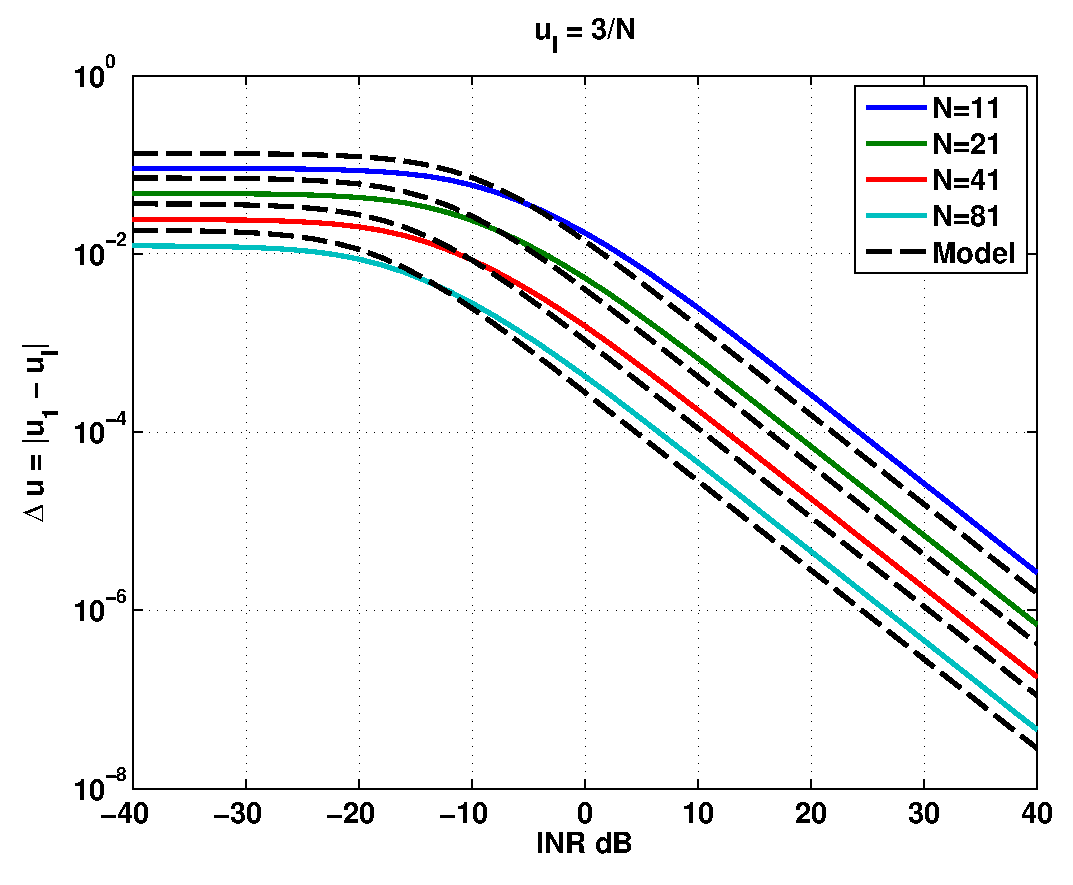
\includegraphics[width=3.5in]{zero_pertb_true_model_ulook1}%
\label{fig:compare_first_case}}

\subfloat[]{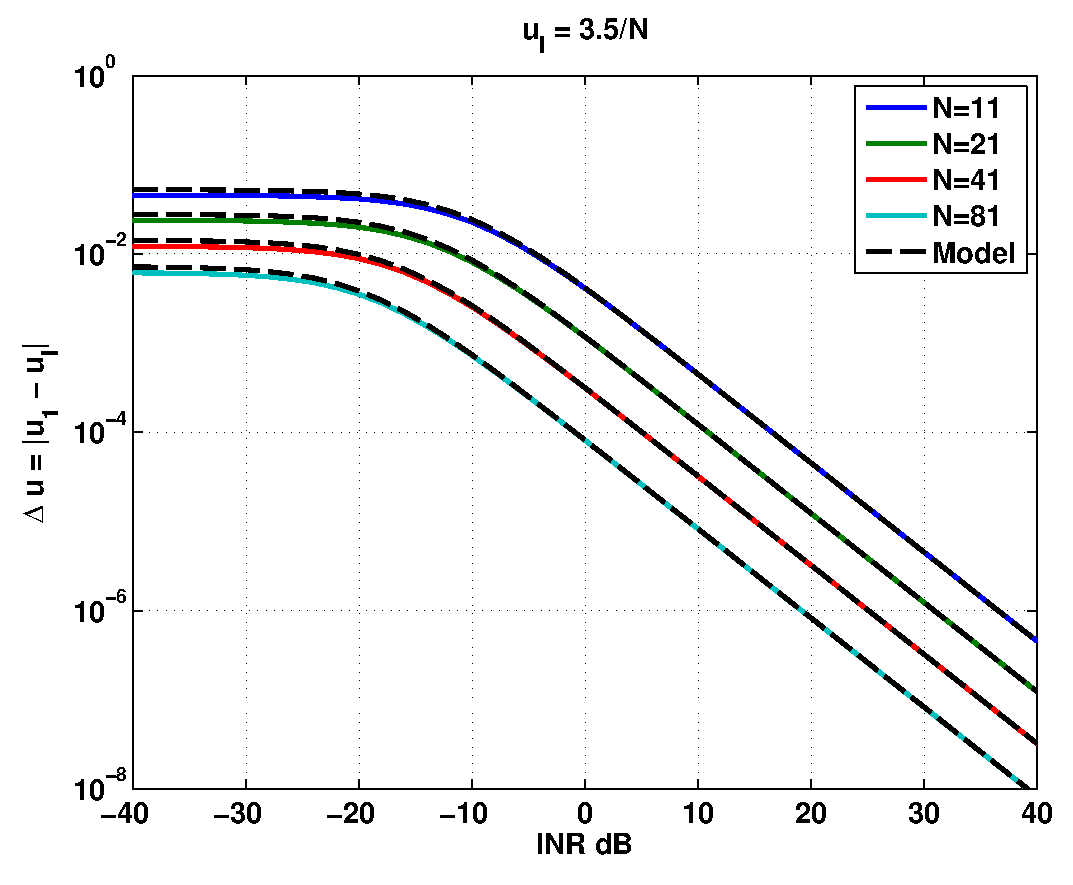
\includegraphics[width=3.5in]{zero_pertb_true_model_ulook2}%
  \label{fig:compare_second_case}}
\caption[Comparison between the actual and the model predicted values
  of the phase angle perturbation $\deltau$.]{Comparison between the actual and the model predicted values
  of the phase angle perturbation $\deltau$ when the interferer is
  present at (a) $\uinter = 3/N$ and (b) $\uinter = 3.5/N$. The model
  gives a good prediction of the actual perturbation values.}
\label{fig:model-true-compare}
\end{figure*}

\section{SMI MVDR ABF polynomial}
\label{sec:smi-poly}
The SMI MVDR ABF is the practical realization of the ensemble MVDR
ABF. Each realization of the SMI MVDR ABF has an array polynomial
representation $\smipoly = \ztrans(\wsmi\herm)$. Factoring the SMI
MVDR ABF polynomial in terms of its zeros
\[
\smipoly = G\prod\limits_{n = 1}^{N-1}(1 - \sampz_nz\inv),
\]
where $G$ is a scaling factor ensuring unity gain in the look
direction ($\ulook$), i.e., $P_S(\expo{j\pi\ulook}) = 1$ and
$\sampz_n$ is the $n\nth$ zero. The SMI MVDR ABF polynomial zeros
($\sampz_n$) will be referred to as sample zeros in the sequel. Each
realization of the SMI MVDR ABF produces a new set of $N-1$ sample
zeros. In addition, the sample zeros ($\sampz_n$) do not necessarily
fall on the unit circle, unlike the ensemble zeros ($\ensz_n$) as
described in \sect{}~\ref{sec:mvdr-interf-suppr}.

Numerical experiments show that the sample zeros ($\sampz_n$) are
randomly perturbed from the ensemble zeros ($\ensz_n$) on the complex
plane. \figurename{}~\ref{fig:smi-mvdr-pzplot} shows sample zeros
(green markers) obtained from 1000 independent realizations of the SMI
MVDR ABF. The blue circle markers denote the ensemble zero
locations. The ABF is implemented using a $N = 11$ sensor ULA and
$L = 110$ snapshot data. A single interferer is present at
$\uinter = 3/N$ with $40$ dB INR. Each green marker denotes one of the
ten sample zeros generated from each realization of the SMI MVDR
ABF. The sample zeros cluster around the ensemble zero locations while
not necessarily falling on the unit circle. The sample zeros appear to
be a zero mean perturbation of the ensemble zero locations, although
no analytical characterization is presented here. The number of
snapshots considered in the example is impractically large for passive
sonar scenario, but it is chosen to enhance the clustering of the
sample zeros.% around the ensemble locations.

The sample zeros located away form the unit circle do not produce
beampattern nulls. Following the analogy with the DT LTI filters, the
sample zeros that fall away from the unit circle produce shallow
troughs instead of deep nulls in the beampattern. Moreover sample
zeros that fall closer to the origin or far outside the unit circle
have negligible contribution to beampattern
\cite[Chap.~5]{Oppenheim1989}. Hence SMI MVDR ABF suffers from high
sidelobes and a distorted mainlobe in the beampattern. Consequently,
the SMI MVDR ABF loses ability to suppress interferers and white
noise. The following chapter describes how the SMI MVDR ABF can be
modified to improve interferer suppression by projecting the sample
zeros to the unit circle.

%% Add this later after JRB approves other detail
% The SMI MVDR ABF converges in probability to the ensemble
% MVDR ABF as the number of snapshots $L$ increases
% \cite{richmond2000nulling}. This implies that the sample zeros
% converge to ensemble zero locations as the number of snapshot
% increases.

\begin{figure}[!hp]
  \centering
  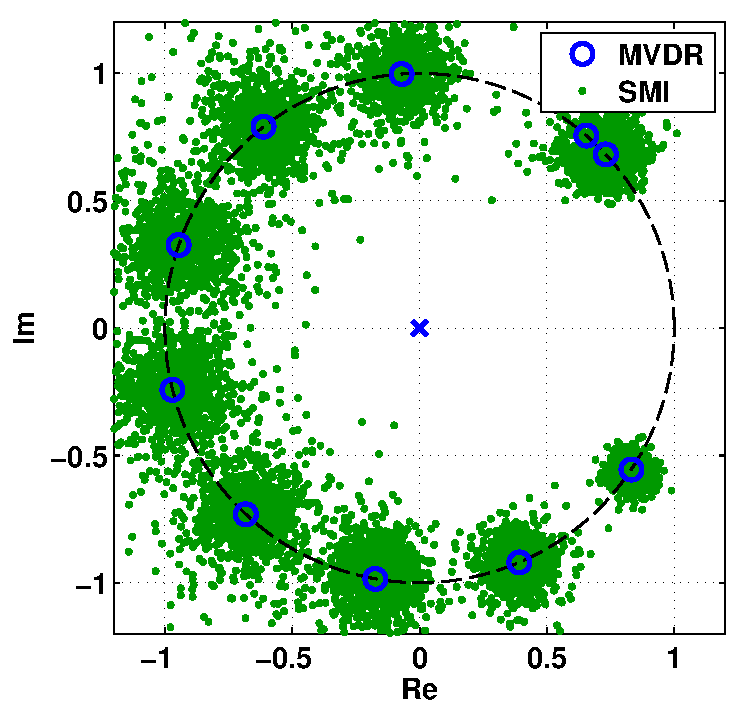
\includegraphics[width=5in]{mvdr_smi_pzlot_N11_L110_INR40}
  \caption[SMI MVDR zeros from 1000 Monte Carlo trials for $N = 11$, $L =
  10 N$ and INR = $40$ dB]{SMI MVDR zeros from 1000 Monte Carlo trials
    for $N = 11$, $L = 10N$ and INR = 40 dB. The dashed radial line
    denotes the phase angle associated with the interferer direction
    $\uinter$. The number of snapshots is impractically large for many
    passive sonar situations, but is chosen to create a clearer
    clustering of the SMI zeroes around the ensemble zeroes.}
  \label{fig:smi-mvdr-pzplot}
\end{figure}

%%% Local Variables:
%%% mode: latex
%%% TeX-master: "main"
%%% End:
